% -*- mode: latex; mode: flyspell; ispell-local-dictionary: "deutsch8" -*-
\documentclass{article}

\def\pgfsysdriver{pgfsys-tex4ht.def}

\usepackage{tikz}
\usetikzlibrary{calc,positioning,chains}

\usepackage{lmodern}

\begin{document}

{\centering
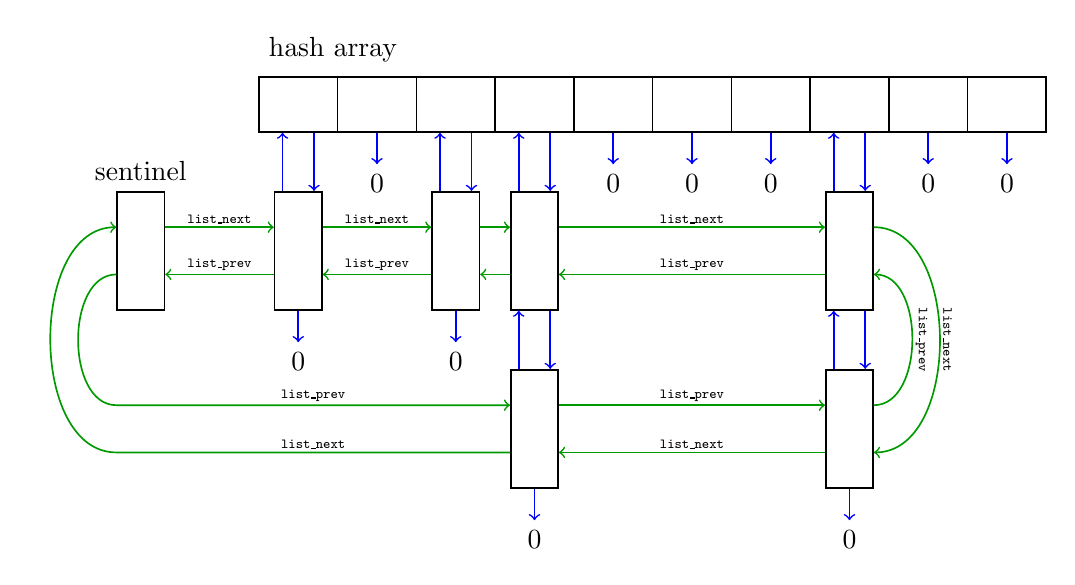
\begin{tikzpicture}[
    semithick,
    box/.style={draw,minimum width=1cm,minimum height=0.7cm},
    boxh/.style={draw,minimum width=0.6cm,minimum height=1.5cm},
    hashline/.style={draw=blue},
    lruline/.style={draw=green!60!black},
    lrunode/.style={above,inner sep=1pt,font=\tt\tiny},
  ]

  \foreach \x in {0,...,9}
    \node (h\x) at (\x,0) [box] {};

  \node at (-0.5,0.7) [right] {hash array};

  % bucket 0
   
  \node (b0-0) at ($(h0.south) + (0,-1.5)$) [boxh] {};

  \draw[hashline,->] ($(h0.south) + (0.2,0)$) -- ($(b0-0.north) + (0.2,0)$);
  \draw[hashline,<-] ($(h0.south) + (-0.2,0)$) -- ($(b0-0.north) + (-0.2,0)$);

  \draw[hashline,->] (b0-0.south) -- +(0,-0.4) node[below] {0};

  % bucket 1

  \draw[hashline,->] (h1.south) -- +(0,-0.4) node[below] {0};

  % bucket 2
    
  \node (b2-0) at ($(h2.south) + (0,-1.5)$) [boxh] {};

  \draw[hashline,->] ($(h2.south) + (0.2,0)$) -- ($(b2-0.north) + (0.2,0)$);
  \draw[hashline,<-] ($(h2.south) + (-0.2,0)$) -- ($(b2-0.north) + (-0.2,0)$);

  \draw[hashline,->] (b2-0.south) -- +(0,-0.4) node[below] {0};

  % bucket 3
   
  \node (b3-0) at ($(h3.south) + (0,-1.5)$) [boxh] {};
  \node (b3-1) at ($(b3-0.south) + (0,-1.5)$) [boxh] {};

  \draw[hashline,->] ($(h3.south) + (0.2,0)$) -- ($(b3-0.north) + (0.2,0)$);
  \draw[hashline,<-] ($(h3.south) + (-0.2,0)$) -- ($(b3-0.north) + (-0.2,0)$);

  \draw[hashline,->] ($(b3-0.south) + (0.2,0)$) -- ($(b3-1.north) + (0.2,0)$);
  \draw[hashline,<-] ($(b3-0.south) + (-0.2,0)$) -- ($(b3-1.north) + (-0.2,0)$);

  \draw[hashline,->] (b3-1.south) -- +(0,-0.4) node[below] {0};

  % bucket 4, 5, 6

  \draw[hashline,->] (h4.south) -- +(0,-0.4) node[below] {0};
  \draw[hashline,->] (h5.south) -- +(0,-0.4) node[below] {0};
  \draw[hashline,->] (h6.south) -- +(0,-0.4) node[below] {0};

  % bucket 7
    
  \node (b7-0) at ($(h7.south) + (0,-1.5)$) [boxh] {};
  \node (b7-1) at ($(b7-0.south) + (0,-1.5)$) [boxh] {};

  \draw[hashline,->] ($(h7.south) + (0.2,0)$) -- ($(b7-0.north) + (0.2,0)$);
  \draw[hashline,<-] ($(h7.south) + (-0.2,0)$) -- ($(b7-0.north) + (-0.2,0)$);

  \draw[hashline,->] ($(b7-0.south) + (0.2,0)$) -- ($(b7-1.north) + (0.2,0)$);
  \draw[hashline,<-] ($(b7-0.south) + (-0.2,0)$) -- ($(b7-1.north) + (-0.2,0)$);

  \draw[hashline,->] (b7-1.south) -- +(0,-0.4) node[below] {0};

  % bucket 8, 9

  \draw[hashline,->] (h8.south) -- +(0,-0.4) node[below] {0};
  \draw[hashline,->] (h9.south) -- +(0,-0.4) node[below] {0};

  % draw sentinel and connect LRU list

  \node (s) at ($(b0-0) + (-2,0)$) [boxh] {};
  \node at (s.north) [above] {sentinel};

  \node (s2) at ($(s.south) + (0,-1.5)$) [boxh,draw=white] {}; % invisible box

  \draw[lruline,->] ($(s.east) + (0,+0.3)$) -- node[lrunode] {list\_next} ($(b0-0.west) + (0,+0.3)$);
  \draw[lruline,<-] ($(s.east) + (0,-0.3)$) -- node[lrunode] {list\_prev} ($(b0-0.west) + (0,-0.3)$);

  \draw[lruline,->] ($(b0-0.east) + (0,+0.3)$) -- node[lrunode] {list\_next} ($(b2-0.west) + (0,+0.3)$);
  \draw[lruline,<-] ($(b0-0.east) + (0,-0.3)$) -- node[lrunode] {list\_prev} ($(b2-0.west) + (0,-0.3)$);

  \draw[lruline,->] ($(b2-0.east) + (0,+0.3)$) -- ($(b3-0.west) + (0,+0.3)$);
  \draw[lruline,<-] ($(b2-0.east) + (0,-0.3)$) -- ($(b3-0.west) + (0,-0.3)$);

  \draw[lruline,->] ($(b3-0.east) + (0,+0.3)$) -- node[lrunode] {list\_next} ($(b7-0.west) + (0,+0.3)$);
  \draw[lruline,<-] ($(b3-0.east) + (0,-0.3)$) -- node[lrunode] {list\_prev} ($(b7-0.west) + (0,-0.3)$);

  \draw[lruline,->] ($(b7-0.east) + (0,+0.3)$) to[out=0,in=0] node[lrunode,sloped] {list\_next} ($(b7-1.east) + (0,-0.3)$);
  \draw[lruline,<-] ($(b7-0.east) + (0,-0.3)$) to[out=0,in=0] node[lrunode,sloped] {list\_prev} ($(b7-1.east) + (0,+0.3)$);

  \draw[lruline,->] ($(b7-1.west) + (0,-0.3)$) -- node[lrunode] {list\_next} ($(b3-1.east) + (0,-0.3)$);
  \draw[lruline,<-] ($(b7-1.west) + (0,+0.3)$) -- node[lrunode] {list\_prev} ($(b3-1.east) + (0,+0.3)$);

  \draw[lruline,->] ($(b3-1.west) + (0,-0.3)$) -- node[lrunode,sloped] {list\_next} ($(s2.west) + (0,-0.3)$) to[out=180,in=180] ($(s.west) + (0,+0.3)$);
  \draw[lruline,<-] ($(b3-1.west) + (0,+0.3)$) -- node[lrunode,sloped] {list\_prev} ($(s2.west) + (0,+0.3)$) to[out=180,in=180] ($(s.west) + (0,-0.3)$);

\end{tikzpicture}
\par}


{\centering
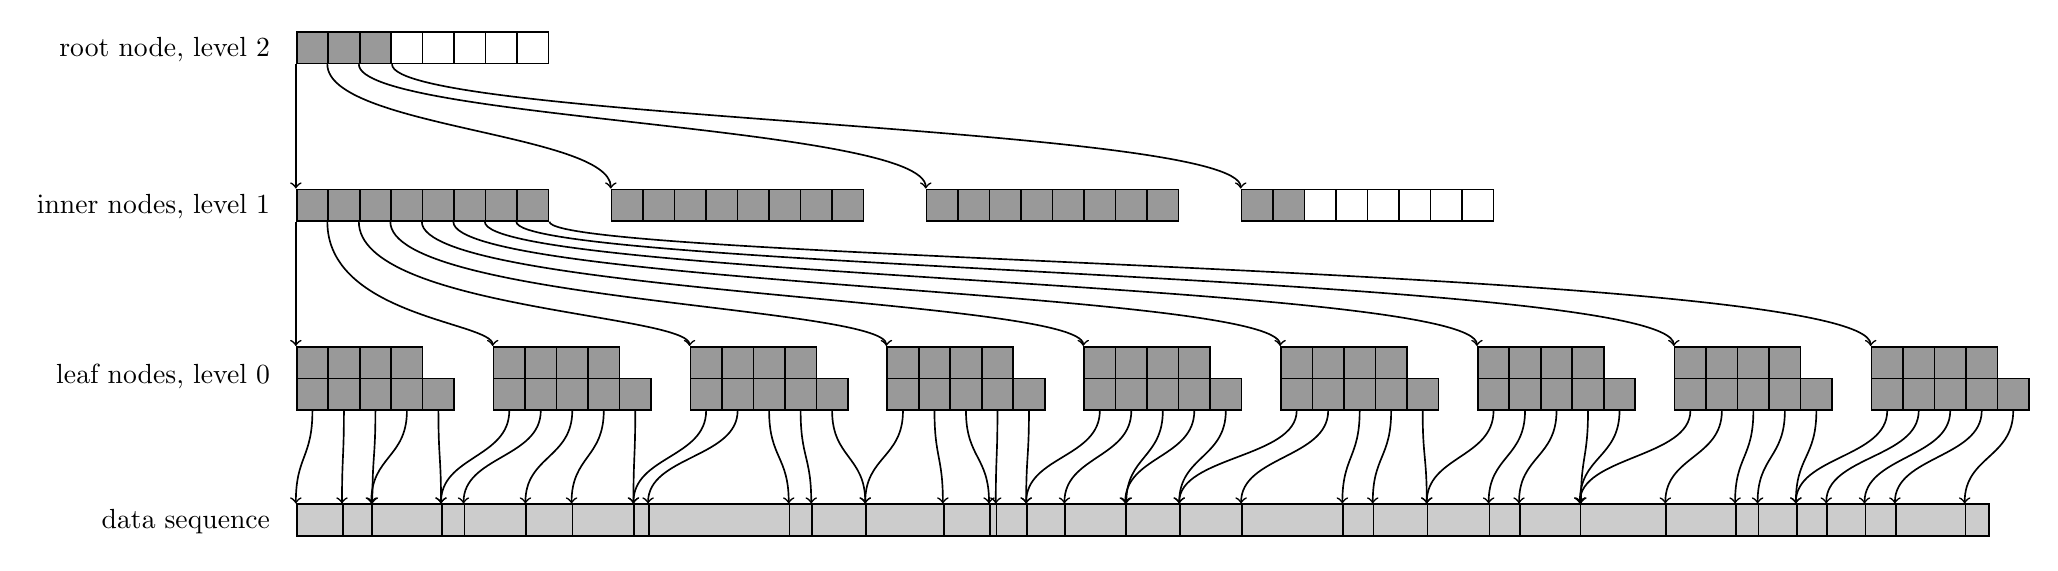
\begin{tikzpicture}[
    semithick,
    box/.style={draw,anchor=west,minimum width=0.4cm,minimum height=0.4cm},
    boxf/.style={box,fill=black!40},
    tnode/.style={above,inner sep=1pt,font=\tt\tiny},
  ]

  \node at (-0.2,-0.02) [left] {root node, level 2};

  \foreach \x in {0,...,2}
  {
    \node (a-\x) at (\x*0.4,0) [boxf] {};
  }
  \foreach \x in {3,...,7}
  {
    \node (a-\x) at (\x*0.4,0) [box] {};
  }

  \node at (-0.2,-2.02) [left] {inner nodes, level 1};

  \foreach \n in {0,...,2}
  {
    \foreach \x in {0,...,7}
    {
      \node (b-\n-\x) at (\x*0.4 + \n*4,-2) [boxf] {};
    }
  }

  { \def\n{3}

    \foreach \x in {0,...,1}
    {
      \node (b-\n-\x) at (\x*0.4 + \n*4,-2) [boxf] {};
    }
    \foreach \x in {2,...,7}
    {
      \node (b-\n-\x) at (\x*0.4 + \n*4,-2) [box] {};
    }
  }

  \draw[->] (a-0.south west) .. controls +(down:0.9cm) and +(up:0.6cm) .. (b-0-0.north west);
  \draw[->] (a-1.south west) .. controls +(down:0.8cm) and +(up:0.7cm) .. (b-1-0.north west);
  \draw[->] (a-2.south west) .. controls +(down:0.7cm) and +(up:0.8cm) .. (b-2-0.north west);
  \draw[->] (a-2.south east) .. controls +(down:0.7cm) and +(up:0.8cm) .. (b-3-0.north west);

  \node at (-0.2,-4.18) [left] {leaf nodes, level 0};

  \foreach \n in {0,...,8}
  {
    \foreach \x in {0,...,3}
      \node (c-\n-\x) at (\x*0.4 + \n*2.5,-4) [boxf] {};

    \foreach \x in {0,...,4}
      \node (co-\n-\x) at (\x*0.4 + \n*2.5,-4.4) [boxf] {};
  }

  \draw[->] (b-0-0.south west) .. controls +(down:1.3cm) and +(up:0.2cm) .. (c-0-0.north west);
  \draw[->] (b-0-1.south west) .. controls +(down:1.2cm) and +(up:0.3cm) .. (c-1-0.north west);
  \draw[->] (b-0-2.south west) .. controls +(down:1.1cm) and +(up:0.4cm) .. (c-2-0.north west);
  \draw[->] (b-0-3.south west) .. controls +(down:1.0cm) and +(up:0.5cm) .. (c-3-0.north west);
  \draw[->] (b-0-4.south west) .. controls +(down:0.9cm) and +(up:0.6cm) .. (c-4-0.north west);
  \draw[->] (b-0-5.south west) .. controls +(down:0.8cm) and +(up:0.7cm) .. (c-5-0.north west);
  \draw[->] (b-0-6.south west) .. controls +(down:0.7cm) and +(up:0.8cm) .. (c-6-0.north west);
  \draw[->] (b-0-7.south west) .. controls +(down:0.6cm) and +(up:0.9cm) .. (c-7-0.north west);
  \draw[->] (b-0-7.south east) .. controls +(down:0.5cm) and +(up:1.0cm) .. (c-8-0.north west);

  \node at (-0.2,-6.02) [left] {data sequence};

  \begin{scope}[yshift=-6cm,start chain,node distance=-1pt,every node/.style={box,inner sep=0pt,on chain,fill=black!20}]
    \node (d-0) [minimum width=0.6cm] {};
    \node (d-1) [minimum width=0.4cm] {};
    \node (d-2) [minimum width=0.0cm] {};
    \node (d-3) [minimum width=0.9cm] {};
    \node (d-4) [minimum width=0.3cm] {};
    \node (d-5) [minimum width=0.8cm] {};
    \node (d-6) [minimum width=0.6cm] {};
    \node (d-7) [minimum width=0.8cm] {};
    \node (d-8) [minimum width=0.2cm] {};
    \node (d-9) [minimum width=1.8cm] {};
    \node (d-10) [minimum width=0.3cm] {};
    \node (d-11) [minimum width=0.7cm] {};
    \node (d-12) [minimum width=1.0cm] {};
    \node (d-13) [minimum width=0.6cm] {};
    \node (d-14) [minimum width=0.1cm] {};
    \node (d-15) [minimum width=0.4cm] {};
    \node (d-16) [minimum width=0.5cm] {};
    \node (d-17) [minimum width=0.8cm] {};
    \node (d-18) [minimum width=0.0cm] {};
    \node (d-19) [minimum width=0.7cm] {};
    \node (d-20) [minimum width=0.8cm] {};
    \node (d-21) [minimum width=1.3cm] {};
    \node (d-22) [minimum width=0.4cm] {};
    \node (d-23) [minimum width=0.7cm] {};
    \node (d-24) [minimum width=0.8cm] {};
    \node (d-25) [minimum width=0.4cm] {};
    \node (d-26) [minimum width=0.8cm] {};
    \node (d-27) [minimum width=0.0cm] {};
    \node (d-28) [minimum width=1.1cm] {};
    \node (d-29) [minimum width=0.9cm] {};
    \node (d-30) [minimum width=0.3cm] {};
    \node (d-31) [minimum width=0.5cm] {};
    \node (d-32) [minimum width=0.4cm] {};
    \node (d-33) [minimum width=0.5cm] {};
    \node (d-34) [minimum width=0.4cm] {};
    \node (d-35) [minimum width=0.9cm] {};
    \node (d-36) [minimum width=0.3cm] {};
  \end{scope}

  \foreach \l in {0,...,8}
  {
    \foreach \n in {0,...,4}
    {
      \pgfmathtruncatemacro{\t}{4*\l + \n}
      \draw[->] (co-\l-\n.south) .. controls +(down:0.6cm) and +(up:0.6cm) .. (d-\t.north west);
    }
  }

\end{tikzpicture}
\par}

\end{document}


